\section{Convergence Plots}
\begin{center}
	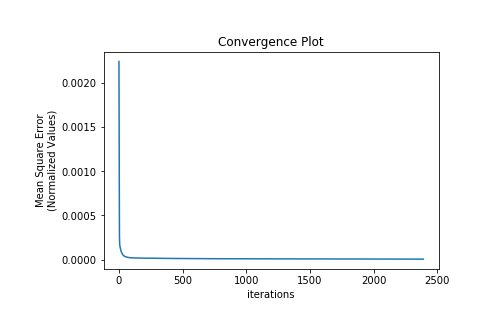
\includegraphics{images/Convergence/Convergence_Plot.png}
	\captionof{figure}{Convergence plot}
\end{center}
The convergence plot is for the selected parameters i.e. No. of hidden neurons = 20, Learning Rate = 0.9, Momentum Coefficients = 0.6 and error/Tolerance = $5\times10^{-6}$. From the convergence plot is can be seen that for the first few iterations, around 5-10, there is major drop in the Mean Square Error(MSE) and after that the curve seems to be flat. To better visualize how the error is reducing after these iterations two more convergence plots are shown in figure 3.2 and figure 3.3.\\
\begin{center}
	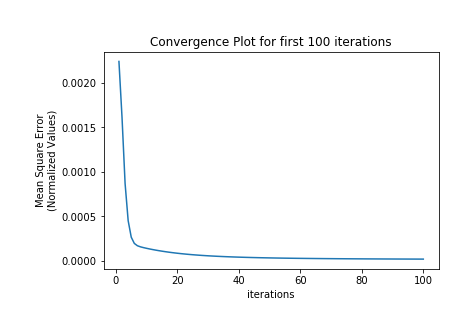
\includegraphics[scale=0.8]{images/Convergence/Convergence_Plot1.png}
	\captionof{figure}{Convergence Plot for first 100 iterations}
\end{center}
From figure 3.2 it can be seen that the reduction in error is very high in first few iterations and around 20 iterations it seems as if the curve is flattening. As the weight values at the start are random the error is high and as the training is proceding the error is reducing.
\begin{center}
	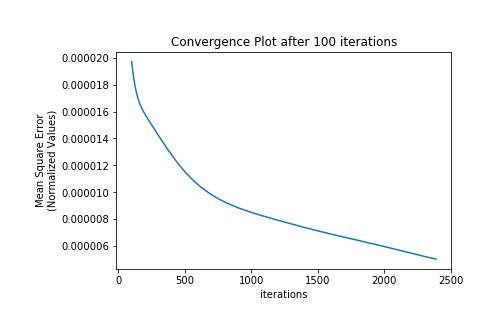
\includegraphics[scale=0.8]{images/Convergence/Convergence_Plot2.png}
	\captionof{figure}{Convergence Plot after 100 iterations}
\end{center}
From figure 3.3 we can appreciate how the error is reducing continuously and the curve actually do not go flat. Even at termination condition curve is quite steep and with further reduction in tolerance value of termination the MSE will further reduce.

\section{Predictions}
\begin{center}
	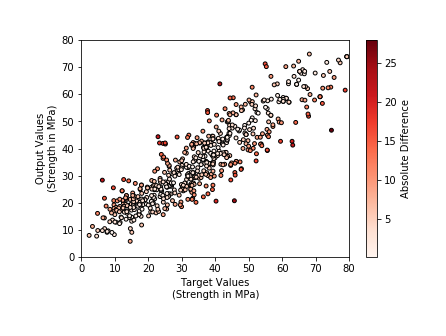
\includegraphics{images/comparison.png}
	\captionof{figure}{Comparison of Target values and Output Values}
\end{center}
Plot in figure 3.4 shows that the prediction values are close to the target values. Variation of Absolute difference between predicted and target values is same throughout. So it cannot be concluded if the method is better for low strength or high strength high-performance concrete. Also the model is Underpredicting and overpredicting by same amount as it can be see by the color which is similar on both sides of portion of the graph with white points.
\begin{center}
	\begin{tabular}{|c|c|}
		\hline
		Maximum absolute Error & 27.9126\\
		\hline
		Minimum absolute Error & 0.0155\\
		\hline
		Mean absolute Error & 5.7182\\
		\hline
		Mean square Error & 52.9724\\
		\hline
	\end{tabular}
	\captionof{table}{Errors in Training Ouput}
\end{center}
\begin{center}
	\begin{tabular}{|c|c|}
		\hline
		Maximum absolute Error & 22.3789\\
		\hline
		Minimum absolute Error & 0.01622\\
		\hline
		Mean absolute Error & 5.3483\\
		\hline
		Mean square Error & 48.7034\\
		\hline
	\end{tabular}
	\captionof{table}{Errors in Testing Ouput}
\end{center}
Tables 3.1 and 3.2 shows various errors in prediction by the ANN Model for training and testing respectively. For both cases the values of errors are almost similar indicating the model has not over-fitted the training data. The maximum absolute error in both cases is high.

\section{Comparison}
In this section a comparison is made between the Model with selected parameters and a model with same parameters and lower tolerance i.e. $10^{-6}$. Though the reduction is only of $5\times10^{-6}$ it will lead to some intersing results.
\subsection{Convergence Plots}
Similar to the section 3.1 here 3 convergece plots are shown in figure 3.5.
\begin{center}
	\begin{tabular}{c}
		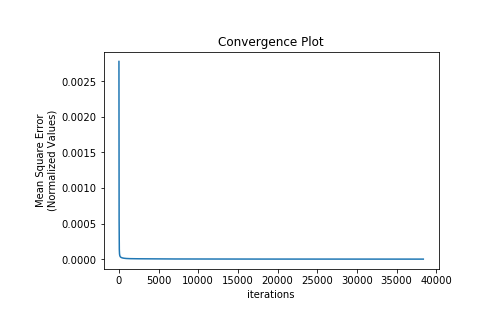
\includegraphics[scale=0.65]{images/comparison/Convergence_Plot_a.png}\\
		a)\\
	\end{tabular}
	\begin{tabular}{cc}
		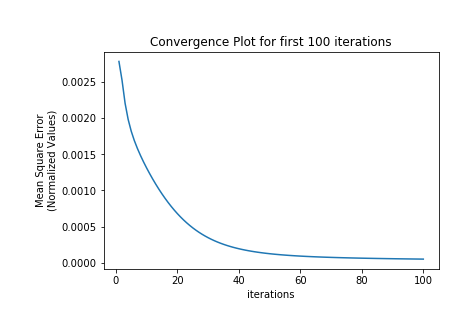
\includegraphics[scale=0.5]{images/comparison/Convergence_Plot1_a.png} & 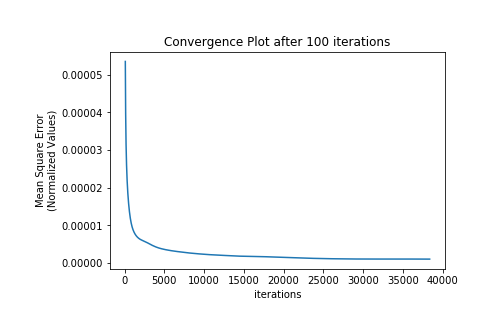
\includegraphics[scale=0.5]{images/comparison/Convergence_Plot2_a.png}\\
		b) & c)\\
	\end{tabular}
	\captionof{figure}{Convergence Plot for a) All iteration; b) First 100 iterations; c) After 100 iterations}
\end{center}
In figure 3.4 a) similar trend can seen in the plot that were seen in figure 3.1. The convergence rate is high in the starting and then it is low as the error is reduced to around $4\times10^{-5}$.\\
From figure 3.5 b) for first 100 iteraton trend is also same that the curve is flattening as the number of iterations are increasing. After 100 iterartions the trend in starting of figure 3.5 c) is similar to figure 3.3 but there is a change in the later stage. At 5000 iterations the error is $3\times10^{-6}$ and after that there is not much change in error and convergence rate is very low and it takes total of 38373 iterations for termination criterion to be fulfiled i.e. $MSE<10^{-6}$. The curve is almost flat in this case while for that in figure 3.3 the curve was quite steep.

\subsection{Predictions}
\begin{center}
	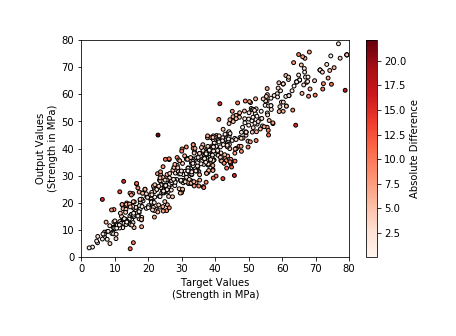
\includegraphics[scale=0.8]{images/comparison/comparison_a.png}
	\captionof{figure}{Comparison of Target values and Output Values}
\end{center}
Plot in figure 3.6 shows that the prediction values are close to the target values. Points are more close to $y=x$ line than in figure 3.4 and also the colors are not as dark for the values.
This implies that most of the predictions are close to the targets and there are lesser number of values which are far from target. This can also be seen from the tables 3.3 and 3.4 that there is a reduction in Mean Square Error and Mean Absolute Error.
\begin{center}
	\begin{tabular}{|c|c|}
		\hline
		Maximum absolute Error & 22.11\\
		\hline
		Minimum absolute Error & 0.005\\
		\hline
		Mean absolute Error & 3.7328\\
		\hline
		Mean square Error & 23.69096\\
		\hline
	\end{tabular}
	\captionof{table}{Errors in Training Ouput}
\end{center}
\begin{center}
	\begin{tabular}{|c|c|}
		\hline
		Maximum absolute Error & 24.924\\
		\hline
		Minimum absolute Error & 0.0625\\
		\hline
		Mean absolute Error & 4.3087\\
		\hline
		Mean square Error & 32.4043\\
		\hline
	\end{tabular}
	\captionof{table}{Errors in Testing Ouput}
\end{center}